\documentclass[11pt,a4paper]{report}

\usepackage[utf8]{inputenc}
\usepackage{amsmath}
\usepackage{graphicx}
\usepackage{gensymb}
\usepackage{tikz}
\usepackage{pgfplots}
\usetikzlibrary{positioning}
\usepackage{geometry}
\geometry{
    left=2cm,
    right=0.64cm,
    top=0.64cm,
    bottom=2cm
}
\usepackage{multicol}
\setlength{\columnsep}{1cm}
\graphicspath{ {images/} }

\begin{document}

\chapter{Semester 2 Examination 2015-2016\\CZ4041 Machine Learning}

\begin{multicols*}{2}

\section{Question 1}
\noindent \textbf{Question 1a}
\noindent Information given in the question:
\begin{itemize}
  \item $P(D) = 0.001$
  \item $P(\sim D) = 0.999$
  \item $P(T_1|D) = 0.9$
  \item $P(T_2|D) = 0.95$
  \item $P(T_1|\sim D) = 0.01$
  \item $P(T_2|\sim D) = 0.1$
\end{itemize}

\begin{equation*}
\begin{split}
P(D|T_1 T_2) &= \frac{P(T_1 | D) P(T_2 | D) P(D)}{P(T_1 T_2)}\\
&= \frac{0.9 \times 0.95 \times 0.001}{P(T_1 T_2)}\\
&= \frac{0.855 \times 10^{-3}}{P(T_1 T_2)}
\end{split}
\end{equation*}

\begin{equation*}
\begin{split}
P(\sim D|T_1 T_2) &= \frac{P(T_1 | \sim D) P(T_2 | \sim D) P(\sim D)}{P(T_1 T_2)}\\
&= \frac{0.01 \times 0.1 \times 0.999}{P(T_1 T_2)}\\
&= \frac{0.999 \times 10^{-3}}{P(T_1 T_2)}
\end{split}
\end{equation*}

\noindent Since $P(\sim D|T_1 T_2) > P(D|T_1 T_2)$, we predict that the patient does not have the disease.\\

\noindent \textbf{Question 1b}

\noindent Let action $a_1$ be the action predicting the patient to have the disease, and action $a_2$ be the action predicting the patient to not have the disease.

$$R(a_1|T_1 T_2) = 1 - P( D | T_1 T_2)$$
$$R(a_2|T_1 T_2) = 1 - P( \sim D | T_1 T_2)$$

\noindent We choose the action with minimum risk. Since $P(\sim D|T_1 T_2) > P(D|T_1 T_2)$, thus $R(a_2|T_1 T_2) < R(a_1|T_1 T_2)$, so the action $a_2$ has lower risk. As a result, we predict that the patient does not have the disease.\\

\noindent \textbf{Question 1c}

\noindent Information given in the question:
\begin{itemize}
  \item $\lambda_{12} = 0.05$
  \item $\lambda_{21} = 1$
\end{itemize}

\noindent Where $\lambda_{12}$ is the lost occur when the action is predict the patient to have disease $a_1$, but the ground truth is the patient do not have the disease $\sim D$. The lost $\lambda_{21}$ is defined in similar way. The risks are:

\begin{equation*}
\begin{split}
R(a_1|T_1 T_2) &= \lambda_{12} P(\sim D | T_1 T_2)\\
&= 0.05 \times \frac{0.999 \times 10^{-3}}{P(T_1 T_2)}\\
&= \frac{0.4995 \times 10^{-3}}{P(T_1 T_2)}
\end{split}
\end{equation*}

\begin{equation*}
\begin{split}
R(a_2|T_1 T_2) &= \lambda_{21} P( D | T_1 T_2)\\
&= 1 \times \frac{0.855 \times 10^{-3}}{P(T_1 T_2)}\\
&= \frac{0.855 \times 10^{-3}}{P(T_1 T_2)}\\
\end{split}
\end{equation*}

\noindent Since $R(a_1|T_1 T_2) < R(a_2|T_1 T_2)$, we predict that the patient has the disease.

\section{Question 2}
\noindent \textbf{Question 2a}

\noindent We define the inputs to Hidden Layer as:

$$X = \begin{bmatrix} X_1 \\ X_2 \end{bmatrix}$$

\noindent The weight from Input Layer to Hidden Layer is:

$$W =
\begin{bmatrix}
w_{13} & w_{23} \\
w_{14} & w_{24}
\end{bmatrix}$$

\noindent The activation function is:

$$
f(u) =
\begin{cases}
1 & u \ge 0\\
-1 & u < 0
\end{cases}
$$

\noindent The output of the Hidden Layer (which is also the input to Output Layer) is:

$$Z = f(W X)$$

\noindent The weight from Hidden Layer to Output Layer is:

$$V =
\begin{bmatrix}
w_{35} & w_{45}
\end{bmatrix}$$

\noindent The output of Output Layer is:

$$y = f(V Z)$$

\noindent For each $X$, we calculate $y$:

\begin{center}
\begin{tabular}{|c | c | c | c |}
\hline
$X_1$ & $X_2$  & $y$ & Predict \\ \hline
2     & -0.5   & 1   & +       \\
1     & 1      & 1   & -       \\
3     & 1      & 1   & -       \\
2     & -2     & -1  & +       \\
1.5   & 2      & 1   & -       \\ \hline
\end{tabular}
\end{center}

\noindent The error rate is $80\%$.\\

\noindent \textbf{Question 2b}

\noindent We define $X$ as:

$$X =
\begin{bmatrix}
2 & -0.5 \\
1 & 1 \\
3 & 1 \\
2 & -2 \\
1.5 & 2
\end{bmatrix}$$

\noindent The pairwise inner products between the five data points is:

$$X X^{T} =
\begin{bmatrix}
4.25 & 1.50 &  5.50 &  5.00  &  2.00\\
1.50 & 2.00 &  4.00 &  0.00  &  3.50\\
5.50 & 4.00 & 10.00 &  4.00  &  6.50\\
5.00 & 0.00 &  4.00 &  8.00  & -1.00\\
2.00 & 3.50 &  6.50 & -1.00  &  6.25
\end{bmatrix}$$

\noindent \textbf{Question 2c}

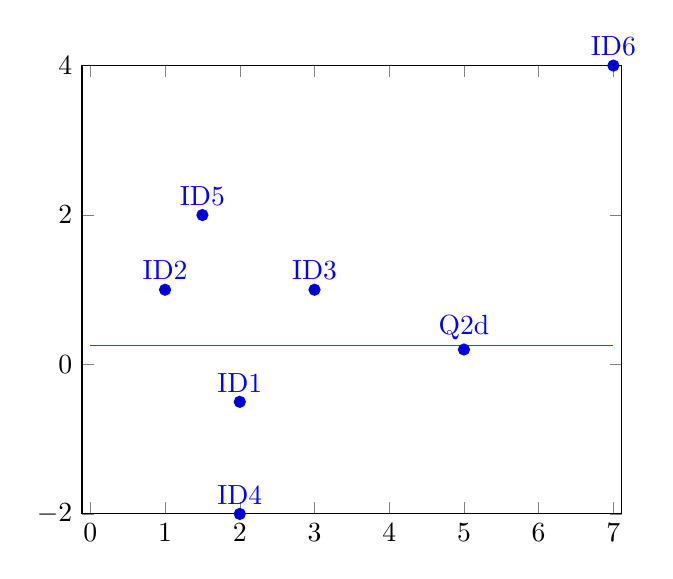
\begin{tikzpicture}
\begin{axis}[
    enlargelimits=false,
    axis equal
]
\addplot+[
    nodes near coords,
    only marks,
    point meta=explicit symbolic
]
table[meta=label] {
    x   y   label
    2  -0.5 ID1
    1   1   ID2
    3   1   ID3
    2  -2   ID4
    1.5 2   ID5
    7   4   ID6
    5   0.2 Q2d
};
\addplot [
    domain=0:7,
    samples=2,
    color=red,
]
{0.25};
\end{axis}
\end{tikzpicture}

\noindent The decision boundary is $y=0.25$.\\

\noindent \textbf{Question 2d}

\noindent Predict the test data point to be + class.

\section{Question 3}

\noindent \textbf{Question 3a}

\noindent If we discard the last eigenvector to reduce the dimension to 2:

$$\text{POV} = \frac{9.78 + 2.11}{9.78 + 2.11 + 0.11} = 0.991$$

\noindent If we discard the last eigenvector to reduce the dimension to 1:

$$\text{POV} = \frac{9.78}{9.78 + 2.11 + 0.11} = 0.815$$

\noindent \textbf{Question 3b}

$$z = U_{\text{reduce}} x^{T}$$
$$U_{\text{reduce}} = \begin{bmatrix}
0.78 & -0.54 & 0.32 \\
0.04 & 0.56 & 0.83
\end{bmatrix}$$

\begin{center}
\begin{tabular}{| c | c | c |}
\hline
Data  & Original    & Reduced\\ \hline
$x_1$ & $(2,0,2)$   & $(2.20,1.74)$   \\
$x_2$ & $(-1,0,-1)$ & $(-1.10,0.87)$  \\
$x_3$ & $(3,-3,0)$  & $(3.96,-1.56)$  \\
$x_4$ & $(-3,2,-2)$ & $(-4.06,-0.66)$ \\
$x_5$ & $(-1,1,1)$  & $(-1.00,1.35)$  \\ \hline
\end{tabular}
\end{center}

\noindent \textbf{Question 3c}

\begin{center}
\begin{tabular}{| c | c  c  c  c  c |} \hline
      & $x_1$  & $x_2$   & $x_3$  & $x_4$  & $x_5$   \\ \hline
$x_1$ & 0      & 3.4128  & 3.7400 & 6.7043 & 3.2237  \\
$x_2$ & 3.4128 & 0       & 5.6132 & 3.3320 & 0.49031 \\
$x_3$ & 3.7400 & 5.6132  & 0      & 8.0703 & 5.7506  \\
$x_4$ & 6.7043 & 3.3320  & 8.0703 & 0      & 3.6611  \\
$x_5$ & 3.2237 & 0.49031 & 5.7506 & 3.6611 & 0       \\ \hline
\end{tabular}
\end{center}

\noindent We merge $x_2$ and $x_5$:

\begin{center}
\begin{tabular}{| c | c  c  c  c  |} \hline
               & $x_2 \cap x_5$  & $x_1$   & $x_3$  & $x_4$  \\ \hline
$x_2 \cap x_5$ & 0               & 3.2237  & 5.6132 & 3.3320 \\
$x_1$          & 3.2237          & 0       & 3.7400 & 6.7043 \\
$x_3$          & 5.6132          & 3.7400  & 0      & 8.0703 \\
$x_4$          & 3.3320          & 6.7043  & 8.0703 & 0      \\ \hline
\end{tabular}
\end{center}

\noindent We merge $x_2 \cap x_5$ with $x_1$:

\begin{center}
\begin{tabular}{| c | c  c  c |} \hline
                        & $x_2 \cap x_5 \cap x_1$ & $x_3$  & $x_4$  \\ \hline
$x_2 \cap x_5 \cap x_1$ & 0                       & 3.7400 & 3.3320 \\
$x_3$                   & 3.7400                  & 0      & 8.0703 \\
$x_4$                   & 3.3320                  & 8.0703 & 0      \\ \hline
\end{tabular}
\end{center}

\noindent We merge $x_2 \cap x_5 \cap x_1$ with $x_4$:


\begin{center}
\begin{tabular}{| c | c  c |} \hline
                                 & $x_2 \cap x_5 \cap x_1 \cap x_4$ & $x_3$  \\ \hline
$x_2 \cap x_5 \cap x_1 \cap x_4$ & 0                                & 3.7400 \\
$x_3$                            & 3.7400                           & 0      \\ \hline
\end{tabular}
\end{center}

\noindent Finally we merge $x_3$ to $x_2 \cap x_5 \cap x_1 \cap x_4$.

\begin{tikzpicture}[sloped]
\node (a) at (0,0) {a};
\node (b) at (1,0) {b};
\node (c) at (2,0) {c};
\node (d) at (3,0) {d};
\node (e) at (4,0) {e};
\node (dummy) at (3.5,5) {};

\node (ab)    at (0.5,0.4903) {};
\node (abc)   at (1.5,3.00) {}; % change the value abit from 3.22
\node (abcd)  at (2.5,3.30) {};
\node (abcde) at (3.5,3.74) {};

\draw  (a)    |- (ab.center);
\draw  (b)    |- (ab.center);
\draw  (ab)   |- (abc.center);
\draw  (c)    |- (abc.center);
\draw  (abc)  |- (abcd.center);
\draw  (d)    |- (abcd.center);
\draw  (abcd) |- (abcde.center);
\draw  (e)    |- (abcde.center);
\draw (abcde) |- (dummy.center);

\end{tikzpicture}

\noindent \textbf{Question 3d}
\noindent [Help wanted!]\\

\section{Question 4}

\noindent \textbf{Question 4a}
\noindent [Copied and pasted from lecture notes] Steps:
\begin{itemize}
\item Train C1 with dataset D1
\item Test C1 with dataset D2
\item Find error samples and an equal amount of correct samples and form D3
\item Train C2 with dataset D3
\item Find error samples and equal amount of correct samples and form D4
\item Train C1and C2 with dataset D4
\item Find errors and equal number of correct samples and form D5
\item Train C3 with D5...
\end{itemize}

\noindent \textbf{Question 4b}
\noindent [Help wanted!]\\

\noindent \textbf{Question 4c i}

\begin{equation*}
\begin{split}
P(A) &= \sum_{B,E} P(A,B,E)\\
     &= \sum_{B,E} P(A | B,E) P(B,E)\\
     &= \sum_{B,E} P(A | B,E) P(B) P(E)\\
     &=       P(A |      B,     E) P(     B) P(     E) +\\
     &\ \ \ \ P(A |      B,\sim E) P(     B) P(\sim E) +\\
     &\ \ \ \ P(A | \sim B,     E) P(\sim B) P(     E) +\\
     &\ \ \ \ P(A | \sim B,\sim E) P(\sim B) P(\sim E)\\
     &=       0.95 \times 0.01 \times 0.02 +\\
     &\ \ \ \ 0.90 \times 0.01 \times 0.98 +\\
     &\ \ \ \ 0.25 \times 0.99 \times 0.02 +\\
     &\ \ \ \ 0.01 \times 0.99 \times 0.98  \\
     &= 0.02366\\
P(\sim A) &= 0.9763
\end{split}
\end{equation*}

\noindent \textbf{Question 4c ii}

\begin{equation*}
\begin{split}
P(S) &= \sum_{A} P(S,A)\\
     &= \sum_{A} P(S|A)P(A)\\
     &=      P(S|     A)P(     A) +\\
     &\ \ \ \ P(S|\sim A)P(\sim A)\\
     &= 0.70 \times 0.02366 + 0.05 \times 0.9763\\
     &= 0.06538
\end{split}
\end{equation*}

\noindent \textbf{Question 4c iii}

\begin{equation*}
\begin{split}
P(S|B) &= \sum_{A} P(S,A|B)\\
       &= \sum_{A} \frac{P(S,A,B)}{P(B)}\\
       &= \sum_{A} \frac{P(S|A,B)P(A,B)}{P(B)}\\
       &= \sum_{A} \frac{P(S|A,B)P(A|B)P(B)}{P(B)}\\
       &= \sum_{A} P(S|A,B)P(A|B)\\
       &= \sum_{A} P(S|A)P(A|B)\\
       &=      P(S|     A)P(     A|B)+\\
       &\ \ \ \ P(S|\sim A)P(\sim A|B)\\
       &= 0.70 \times P(A|B) + 0.05 \times P(\sim A|B)\\
\end{split}
\end{equation*}

\begin{equation*}
\begin{split}
P(A|B)      &= \sum_{E} P(A,E|B)\\
            &= \sum_{E} \frac{P(A,E,B)}{P(B)}\\
            &= \sum_{E} \frac{P(A|E,B)P(E,B)}{P(B)}\\
            &= \sum_{E} \frac{P(A|E,B)P(E)P(B)}{P(B)}\\
            &= \sum_{E} P(A|E,B)P(E)\\
            &= P(A|E,B)P(E) + P(A|\sim E,B)P(\sim E)\\
            &= 0.95 \times 0.02 + 0.90 \times 0.98\\
            &= 0.901\\
P(\sim A|B) &= 0.099\\
P(S|B)      &= 0.70 \times 0.901 + 0.05 \times 0.099\\
            &= 0.6357
\end{split}
\end{equation*}

\begin{equation*}
\begin{split}
P(B|S) &= \frac{P(S|B)P(B)}{P(S)}\\
       &= \frac{0.6357 \times 0.01}{0.06538}\\
       &= 0.09723
\end{split}
\end{equation*}


\end{multicols*}
\end{document}